\section{Theorie}

Das Ziel des Versuches ist es die longitudinale bzw. Spin-Gitter-Relaxationszeit, sowie die
transversale bzw. Spin-Spin-Relaxationszeit von bidestilierten Wasser
mit Hilfe der Kernspinresonanz (NMR) zu bestimmen.

\subsection{Magentisierung im thermischen Gleichgewicht}

Durch das anlegen eines Magnetfeldes werden entarteten Kenspinzustände
der Spinquantenzahl \textbf{I} in $2\text{\textbf{I}} + 1$ äquidistante
Unternivaus aufgespalten.
Die aufgespaltenen Niveaus werden durch die Orientierungsquantenzahl $m$
($-\text{\textbf{I}} \leq m \leq \text{\textbf{I}}$) unterschieden.
Benachbarte Energieniveaus haben einen Abstand von $\Delta E = \gamma B_0\hbar$,
wobei $\gamma$ das gyromagnetische Moment und somit das Verhältnis von
Drehimpuls oder Spin zu dem magnetischen Moment $\vec{\mu}$ darstellt.
Thermisch sind die Energieniveaus gemäß der Boltzmann-Verteilung
besetzt. Das Besetzungsverhältnis zweier benachbarter Energiezustände bei Temperatur $T$
hat folglich die Gestalt
\begin{equation}
  \label{eqn:boltzmann}
  \frac{N(m)}{N(m-1)} = \exp{\left(-\beta(T)\gamma B_0\hbar\right)},\qquad\text{mit }\beta(T) = \frac{1}{k\ua{B}T}.
\end{equation}

Der Erwartungswert der Kernspinpolarisation relativ zu dem angelegten Magnetfeld
$\braket{\text{\textbf{I}}\ua{z}}$ wird gemäß

\begin{equation}
  \label{eqn:erwartung_I}
  \braket{\text{\textbf{I}}\ua{z}} = \frac{\sum_{m = -\text{\textbf{I}}}^\text{\textbf{I}}
  \hbar m \exp{\left(-m\beta(T)\gamma B_0 \hbar\right)}}{\sum_{m = -\text{\textbf{I}}}^\text{\textbf{I}}
  \exp{\left(-m\beta(T)\gamma B_0 \hbar\right)}}
\end{equation}

beschrieben. Die folgenden Rechnungen beschränken sich auf die Vereinfachung
$\text{\textbf{I}} = \frac{1}{2}$, sowie große Magnetfelder $B_0 ~ \SI{1}{\tesla}$.
Dadurch gilt $m\beta(T)\gamma B_0\hbar \ll 1$, weshlab eine Linearisierung der
Exponentialfunktion in Formel~\ref{eqn:erwartung_I} gerechtfertigt ist.
Eine Darstellung der Energieniveaus ist in Abbildung~\ref{fig:proton} zu finden.

\begin{figure}
  \centering
  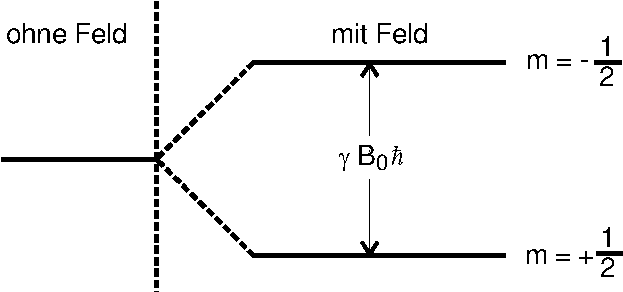
\includegraphics[width = 0.7\textwidth]{Pics/aufspaltungE}
  \caption{Energiezustände eines Protons ($\text{\textbf{I}} = \frac{1}{2}$) im Magnetfeld $B_0$.}
  \label{fig:proton}
\end{figure}

Die Linearisierung von Formel~\ref{eqn:erwartung_I} ergibt
\begin{equation}
  \label{eqn:I_linear}
  \braket{\text{\textbf{I}}_{z} = \frac{1}{2}} = -\frac{\hbar^2}{4}\beta(T)\gamma B_0.
\end{equation}

Die Spinpolarisation führt eine Ausrichtung der mit dem Spin gekoppelten magnetischen
Momente $\vec{\mu}_\text{\textbf{I}}$ mit sich, woher eine makroskopische Magnetisierung
$\vec{M_0}$ rührt.
Liegen $N$ Momente $\vec{\mu}$ in der betrachteten Probe, kann der Betrag der
Magnetisierung $M_0$ geschrieben werden als
\begin{equation}
  \label{eqn:mag}
  M_0 = \frac{1}{4}\mu_0\gamma^2\frac{\hbar^2}N B_0\beta(T).
\end{equation}

\subsection{Lamor-Präzession}
Die magnetischen Momente führen um die Achse des angelegten Magnetfeldes
eine Präzessionsbewegung, welche als Lamor-Präzession bezeichnet wird aus.
Aus der Verbindung zwischen dem Gesamtdrehimpuls und der Magnetisierung
ergibt sich der folgende Zusammenhang.

\begin{equation}
  \label{eqn:mag_diff}
  \frac{\su{d}\vec{M}}{\su{d}t} = \gamma\vec{M}\times B_0\vec{e}_z
\end{equation}

Dabei ist $\vec{e}_z$ der Einheitsrichtungsvektor des Magnetfeldes.
Die Zerlegung von $\vec{M}$ in Einheitsvektoren eines karthesischen Systems
$\vec{e}_x, \vec{e}_y, \vec{e}_z$ führt auf drei Differentialgleichungen.

\begin{align}
  \label{eqn:M_x}
  \frac{\su{d}\vec{M}\cdot \vec{e}_x}{\su{d}t} &= \gamma B_0 \vec{M}\cdot \vec{e}_y, \\
  \label{eqn:M_y}
  \frac{\su{d}\vec{M}\cdot \vec{e}_y}{\su{d}t} &= -\gamma B_0 \vec{M}\cdot \vec{e}_x, \\
  \label{eqn:M_z}
  \frac{\su{d}\vec{M}\cdot \vec{e}_z}{\su{d}t} &= 0
\end{align}

Die Gleichungen~\ref{eqn:M_x}~bis~\ref{eqn:M_z} werden gelöst durch
\begin{align*}
  \vec{M}\cdot \vec{e}_x &= A\cos{(\gamma B_0 t)},\\
  \vec{M}\cdot \vec{e}_y &= -A\sin{(\gamma B_0 t)},\\
  \vec{M}\cdot \vec{e}_z &= \text{const},
\end{align*}
woran erkenntlich wird, dass die Magnetisierung $\vec{M}$ eine Präzession
um $\vec{e}_z$ mit der Lamor-Frequenz $\omega\ua{L} = \gamma B_0$ ausführt.

\subsection{Relaxationserscheinungen}

Relaxation tritt auf, wenn ein System aufgrund einer zeitlich begrenzten
Störung aus dem Gleichgewichtszustand gebracht wird.
In diesem Versuch wird solch eine Störung mit Hilfe hochfreqeunter
Strahlungsquanten realisiert.
Eine Relaxation lässt sich durch eine Abwandlung der Gleichungen~\ref{eqn:M_x}~bis~\ref{eqn:M_z}
mathematisch wie folgt beschreiben

\begin{align}
  \label{eqn:M_x_relax}
  \frac{\su{d}\vec{M}\cdot \vec{e}_x}{\su{d}t} &= \gamma B_0 \vec{M}\cdot \vec{e}_y-\frac{1}{T_2}\vec{M}\cdot \vec{e}_x, \\
  \label{eqn:M_y_relax}
  \frac{\su{d}\vec{M}\cdot \vec{e}_y}{\su{d}t} &= -\gamma B_0 \vec{M}\cdot \vec{e}_x-\frac{1}{T_2}\vec{M}\cdot \vec{e}_y, \\
  \label{eqn:M_z_relax}
  \frac{\su{d}\vec{M}\cdot \vec{e}_z}{\su{d}t} &= \frac{1}{T_1}\left(M_0 - \vec{M}\cdot \vec{e}_z\right).
\end{align}

Die in den Gleichungen auftretenden Zeitkonstanten $T_1$ und $T_2$ sind
verschiedene Relaxationszeiten.
\begin{description}
  \item[Spin-Gitter-Relaxationszeit/longitudinal:]Relaxationszeit parallel zur Magnetfeldrichtung $T_1$.
  Charakteristische Übergangszeit von Energie des Kernspins in Gitterschwingungen und umgekehrt.
  \item[Spin-Spin-Relaxationszeit/transversal:]Relaxationszeit senkrecht zur Magnetfeldrichtung $T_2$.
  Hauptsächlich durch Spinwechselwirkungen mit den nächsten Nachbarn hervorgerufen. Es können
  aber auch Spin-Gitter-Relaxationsprozesse zu $T_2$ beitragen.
\end{description}
